% Phase 1 deck. Build: cd reports && tectonic slides.tex  ->  reports/slides.pdf
% Figures come from reports/figures/ only. Slide owners are noted above each frame.
\documentclass[aspectratio=169,11pt]{beamer}
\usepackage{booktabs}
\usepackage{array}
\usepackage{amsmath}

\definecolor{accent}{HTML}{3D5A80}
\definecolor{muted}{HTML}{5C6670}
\definecolor{tblhead}{HTML}{E9ECEF}

\setbeamercolor{frametitle}{fg=accent}
\setbeamercolor{title}{fg=accent}
\setbeamercolor{structure}{fg=accent}
\setbeamercolor{normal text}{fg=black!85}
\setbeamerfont{frametitle}{size=\Large,series=\bfseries}
\setbeamertemplate{navigation symbols}{}
\setbeamertemplate{itemize items}{\small\raisebox{0.15ex}{$\bullet$}}
\setbeamertemplate{frametitle}{\vspace{0.6em}\insertframetitle\par\vspace{-0.2em}%
  {\color{accent}\rule{2.2cm}{1.2pt}}\par}
\setbeamertemplate{footline}{\hfill{\scriptsize\color{muted}\insertframenumber\,/\,\inserttotalframenumber}\hspace{1.2em}\vspace{0.8em}}
\setlength{\leftmargini}{1.1em}
\graphicspath{{figures/}}

\newcommand{\src}[1]{\par\vfill{\scriptsize\color{muted}#1}}

\title{Next Day Wildfire Spread Prediction}
\subtitle{Phase 1: per-pixel boosted trees with engineered spatial features}
\author{Harshil \and Sushant \and Priyanshu \and Sachin \and Piyush}
\institute{AML course project \quad CS \& AI Department, Rishihood University}
\date{}

\begin{document}

% ---------------------------------------------------------------- Piyush
\begin{frame}[plain]
\vspace{1.5em}
{\color{accent}\Huge\bfseries Next Day Wildfire Spread\\[0.2em] Prediction\par}
\vspace{0.6em}
{\large Phase 1: per-pixel boosted trees with engineered spatial features\par}
\vspace{0.4em}
{\color{accent}\rule{3cm}{1.5pt}\par}
\vspace{1.2em}
Harshil \quad Sushant \quad Priyanshu \quad Sachin \quad Piyush\par
\vspace{0.3em}
{\small\color{muted}AML course project \quad CS \& AI Department, Rishihood University\par}
\vfill
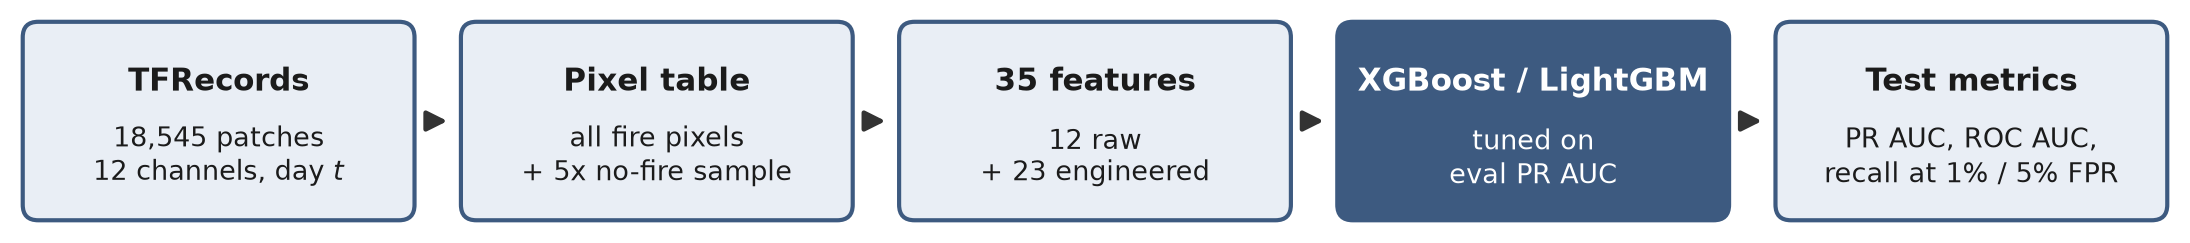
\includegraphics[width=\textwidth]{pipeline.png}
\vspace{0.5em}
\end{frame}

% ---------------------------------------------------------------- Piyush
\begin{frame}{Problem: which pixels burn tomorrow?}
\begin{columns}[T]
\column{0.5\textwidth}
\begin{itemize}
\item Input: 12 channels on day $t$ for a $64\times64$\,km patch at 1\,km (weather, terrain, vegetation, population, today's fire)
\item Output: fire mask on day $t{+}1$, one probability per pixel
\item Only 1.1\% of labelled pixels burn (90:1); cloud or smoke pixels ($-1$) are ignored
\item An all-zero model scores over 98.7\% accuracy, so we report \textbf{PR AUC}: precision and recall on the rare fire class, over all thresholds
\end{itemize}
\column{0.48\textwidth}
\centering
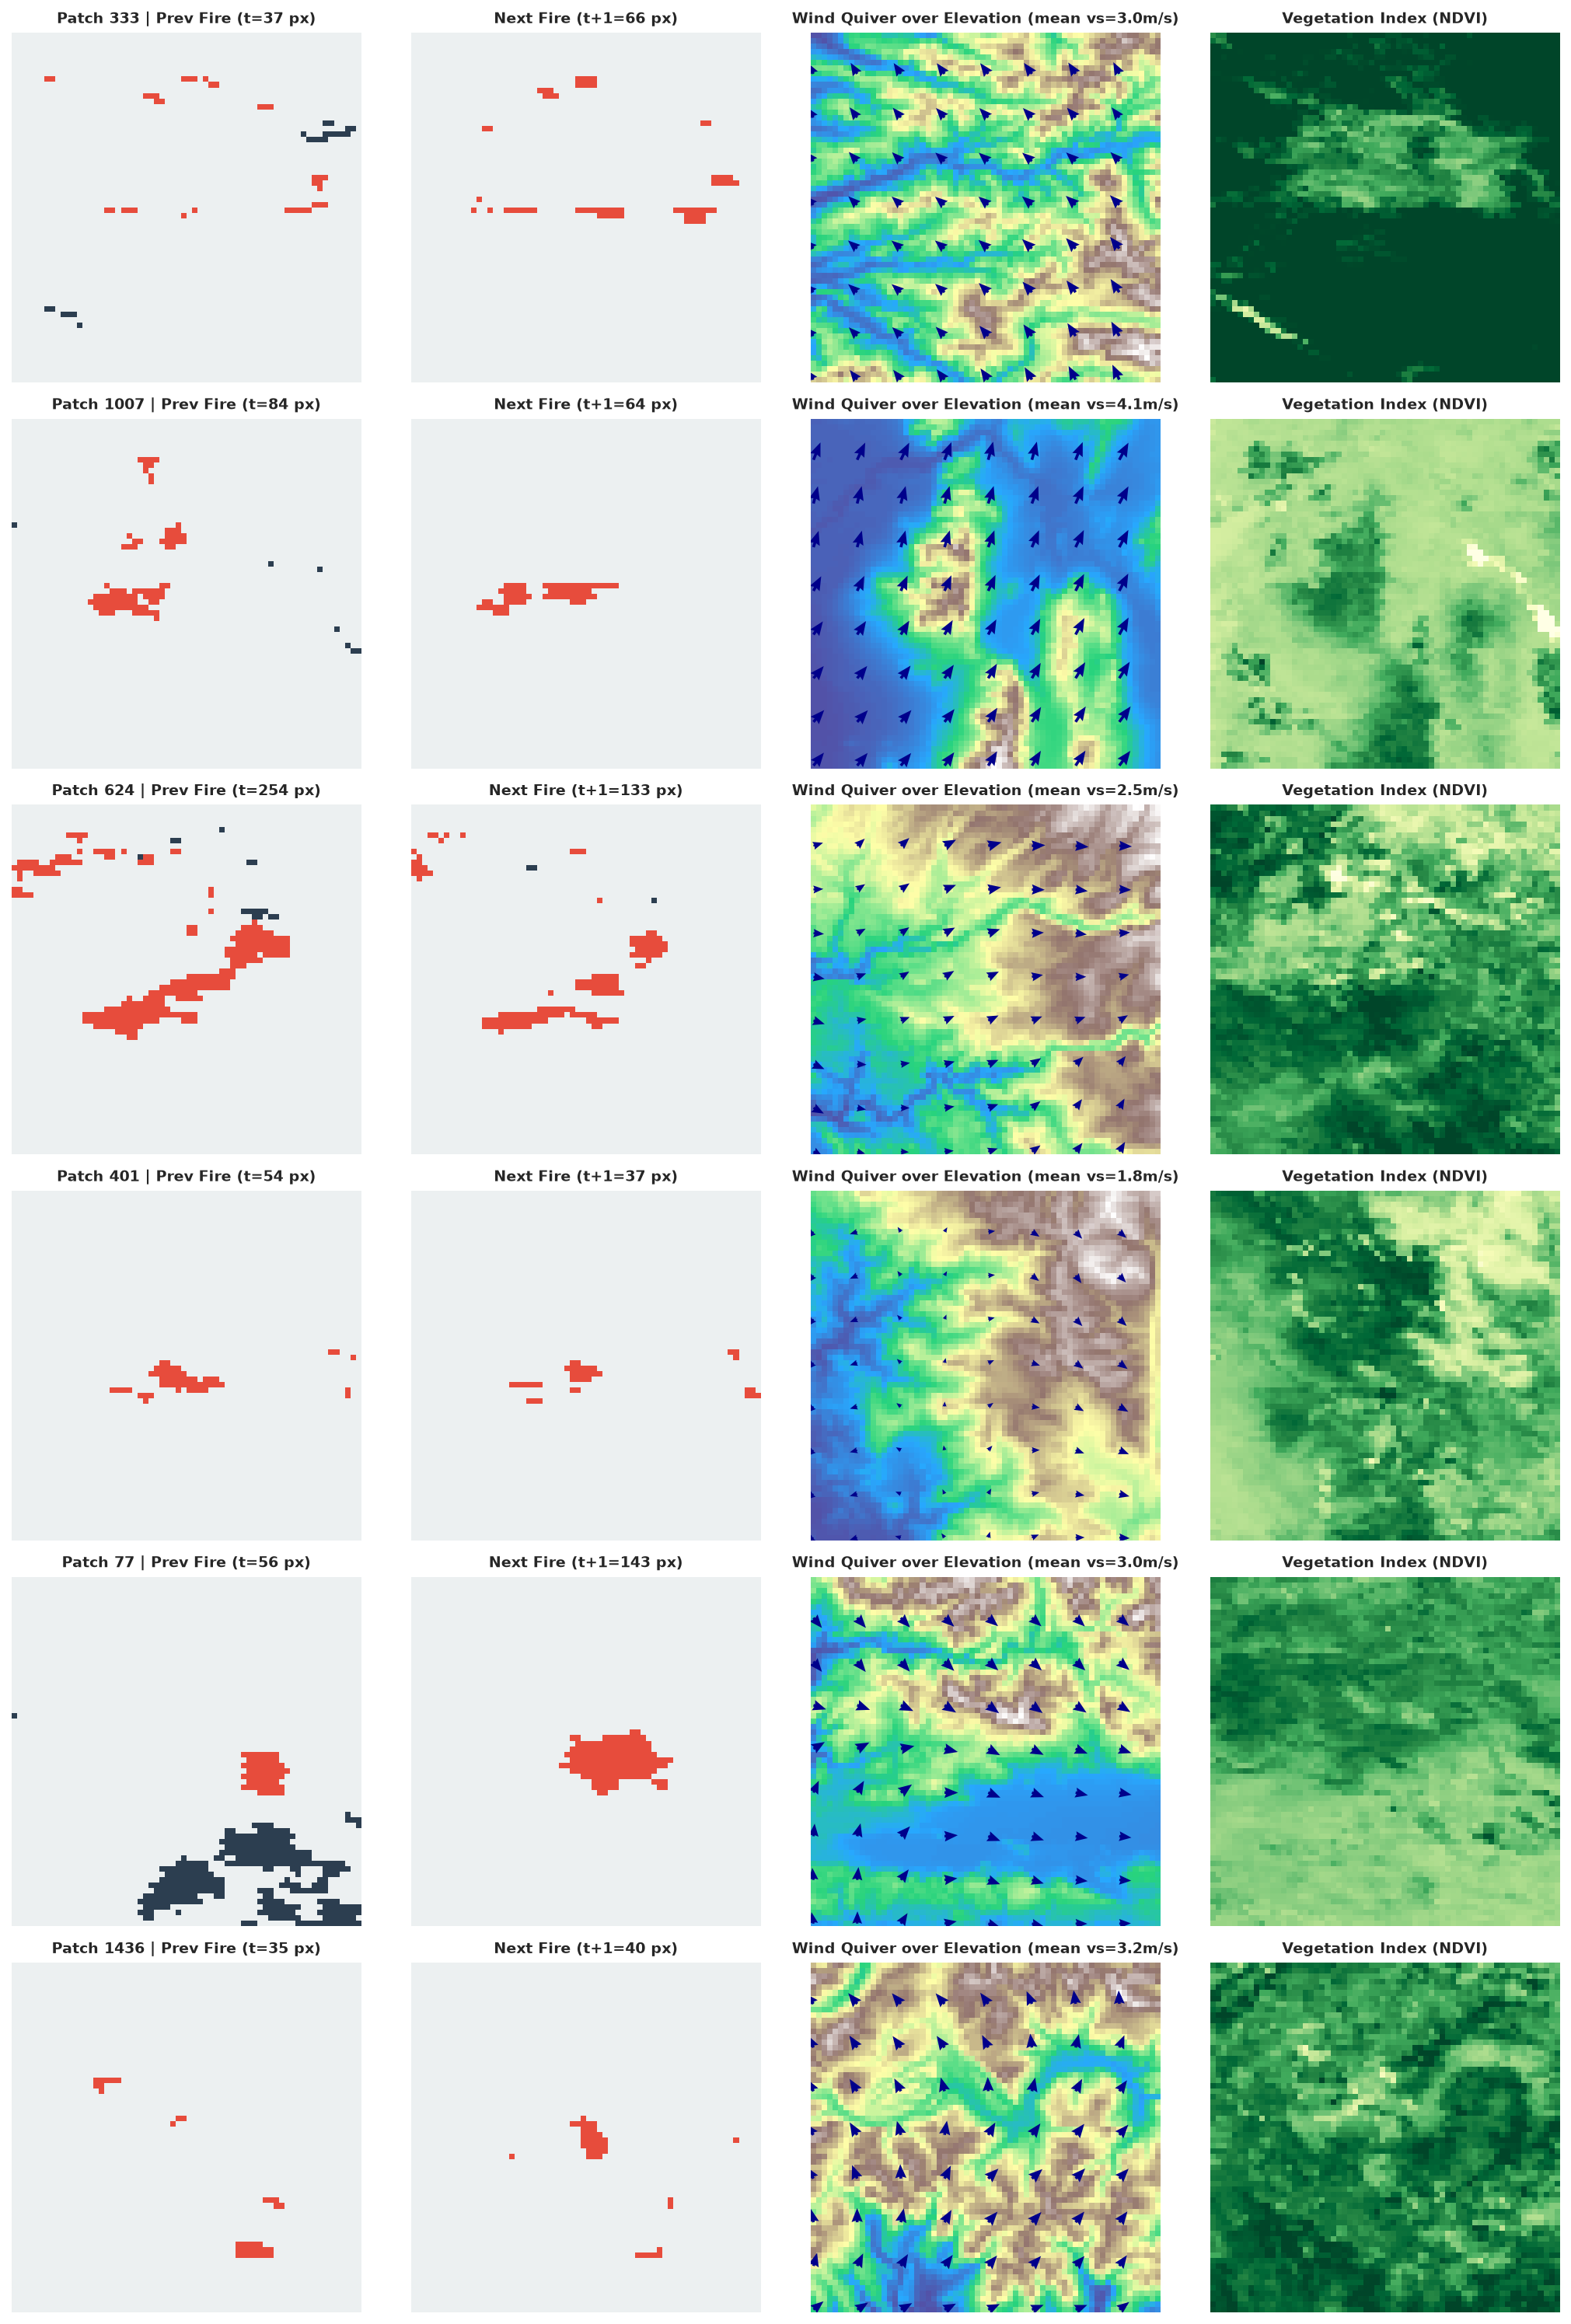
\includegraphics[height=0.62\textheight]{eda_spatial_examples.png}
\end{columns}
\end{frame}

% ---------------------------------------------------------------- Priyanshu
\begin{frame}{Related work at a glance}
\begin{itemize}
\item Other spread models use different data and metrics, so their scores are context only (white rows)
\item Huot et al.\ 2022 built our dataset: their pixel models reach 0.225 PR AUC, the whole-patch CNN 0.284
\item FireCast: 91\% recall but only 3.6\% precision. This is why we report PR AUC, not accuracy
\end{itemize}
\vspace{0.3em}
\centering
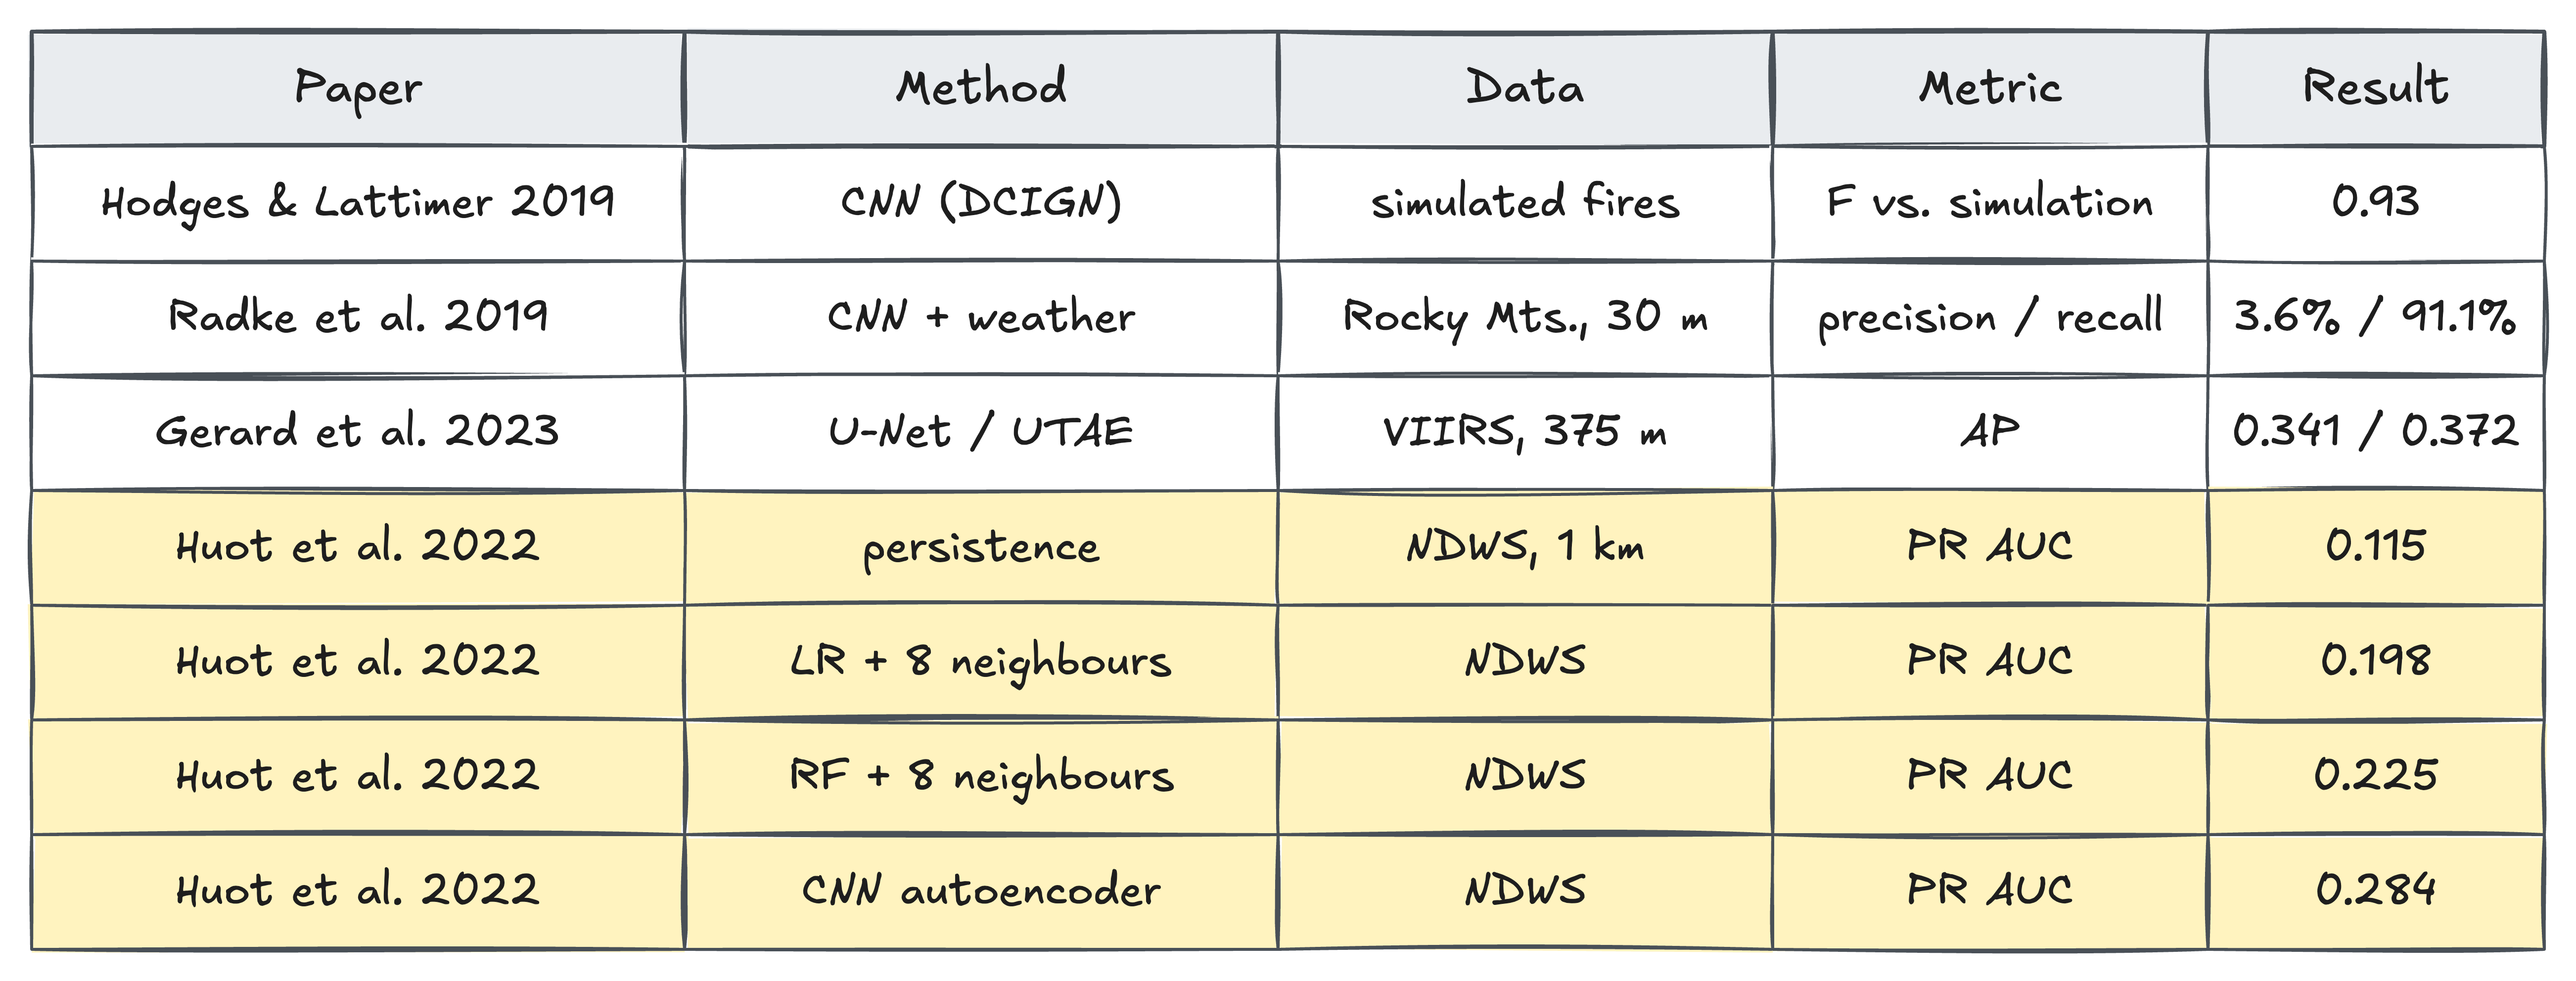
\includegraphics[width=0.7\textwidth]{slide1_related_work_table.png}
\end{frame}

% ---------------------------------------------------------------- Sushant
\begin{frame}{The dataset and why accuracy is useless}
\begin{itemize}
\item 18\,545 patches of US wildfires (2012--2020), $64\times64$\,km at 1\,km, 12 channels on day $t$ $\rightarrow$ fire mask on day $t{+}1$
\item Split by calendar week 8:1:1 with a 1-day buffer: 14\,979 / 1\,877 / 1\,689 patches
\item Next-day fire = 1.1\% of labelled pixels (90:1); an all-zero model scores $>$98.7\% accuracy $\rightarrow$ we report PR AUC
\end{itemize}
\centering
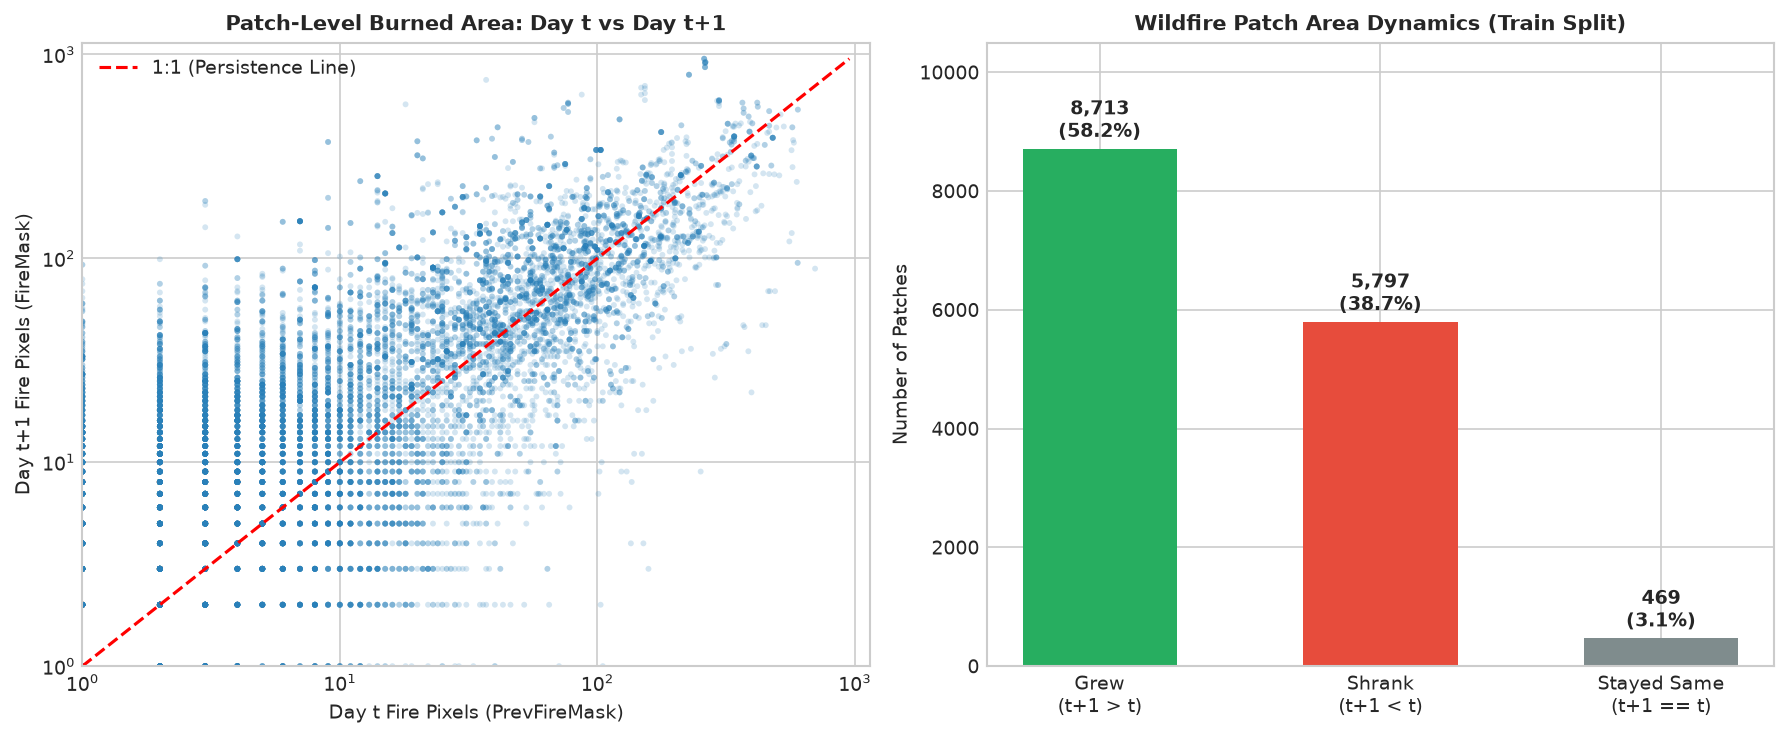
\includegraphics[width=0.66\textwidth]{eda_patch_fire_growth.png}
\src{58\% of fires grow from day $t$ to $t{+}1$, 39\% shrink.}
\end{frame}

% ---------------------------------------------------------------- Sushant
\begin{frame}{What the raw data looks like}
\begin{columns}[T]
\column{0.44\textwidth}
\begin{itemize}
\item Export artefacts: wind direction from $-505\,870^\circ$ to $37\,736^\circ$, temperatures from $-445$\,K to 1\,230\,K, negative rain in 9.8\% of pixels $\rightarrow$ clipped or wrapped
\item ERC (75 vs 54) and elevation (1\,414 vs 709\,m) separate fire from no-fire; wind speed and humidity barely differ
\item Day-$t$ fire has $|\rho| \le 0.09$ with every raw channel $\rightarrow$ the signal is spatial, not in a pixel's own weather
\end{itemize}
\column{0.54\textwidth}
\centering
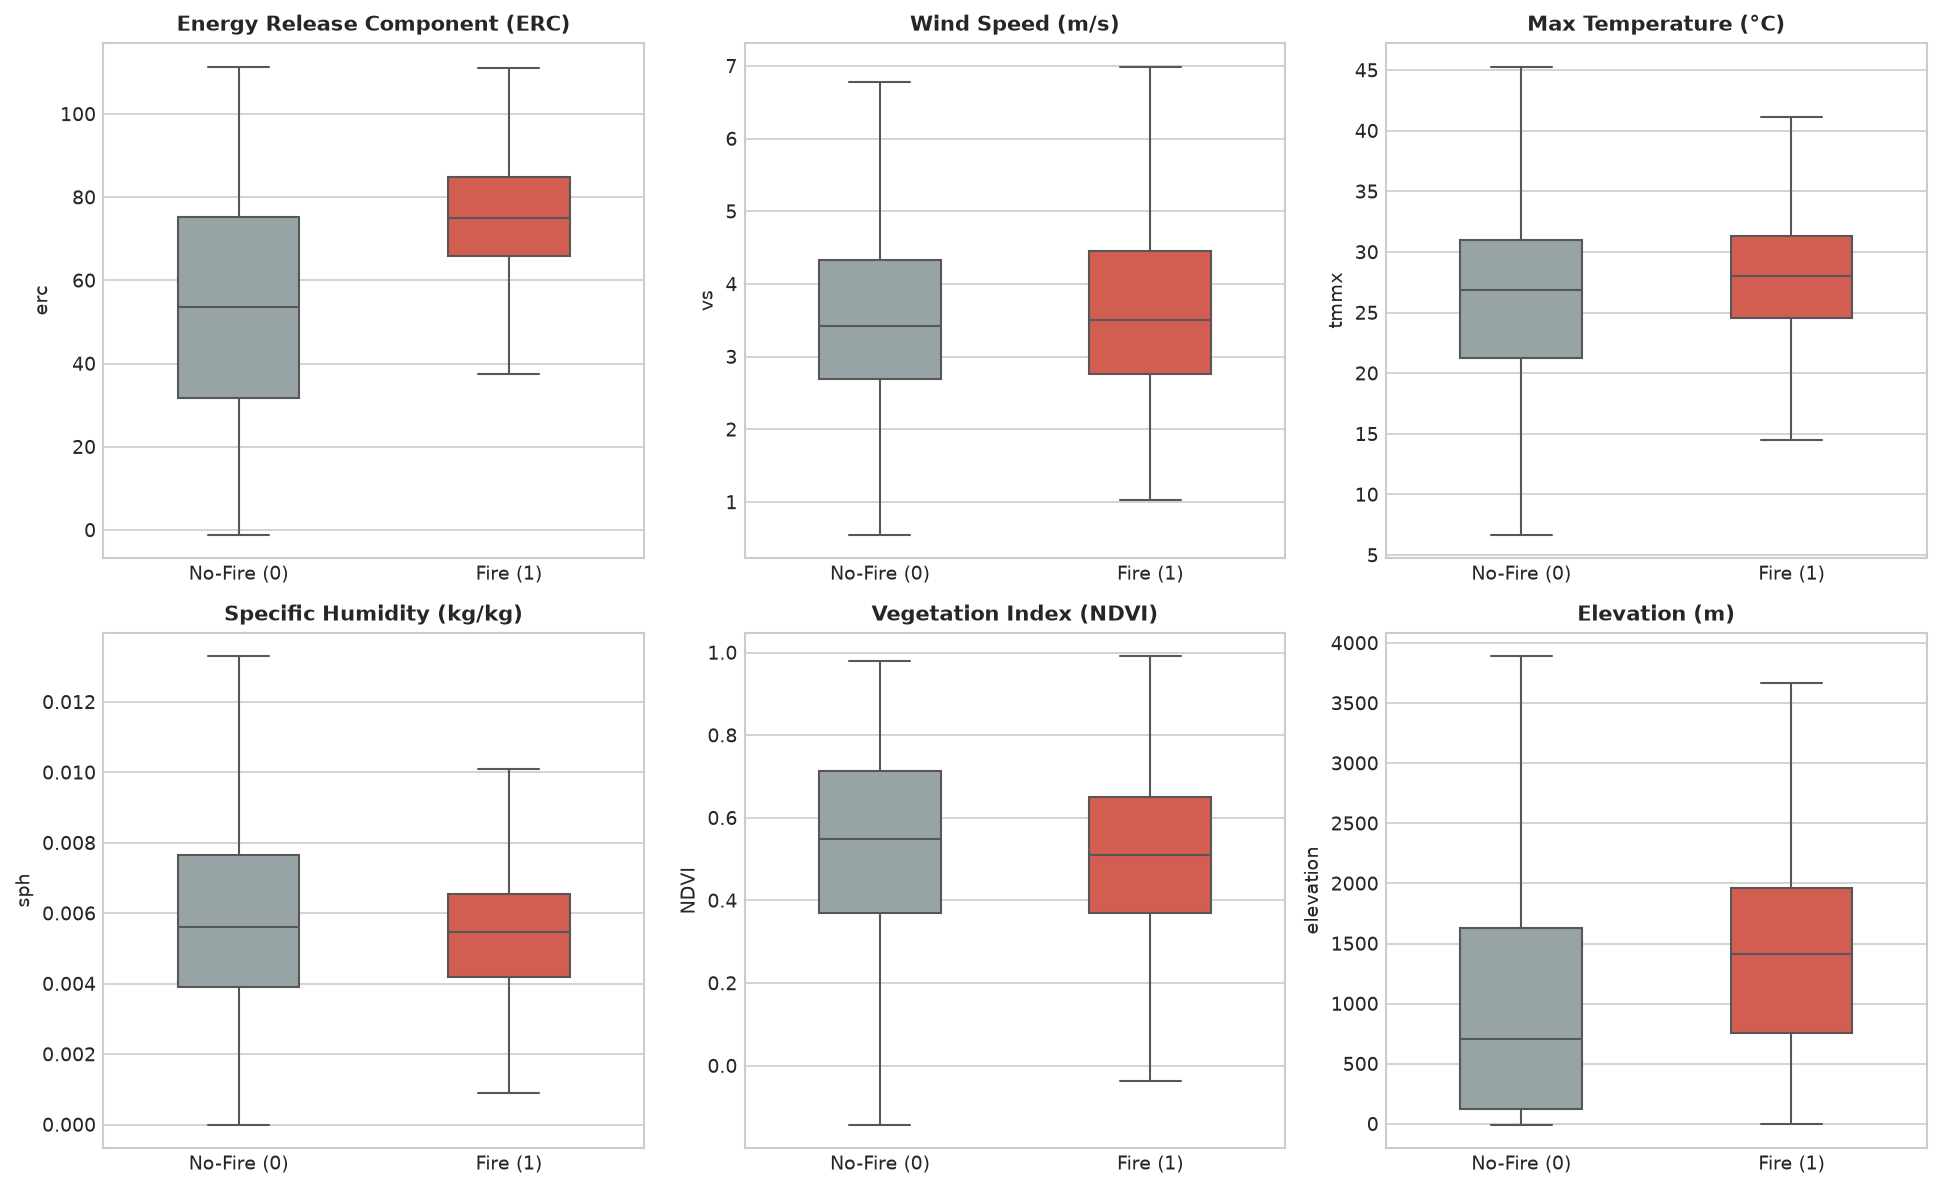
\includegraphics[width=\textwidth]{eda_fire_vs_nofire_features.png}
\end{columns}
\end{frame}

% ---------------------------------------------------------------- Piyush (from paper/sections/methodology.tex)
\begin{frame}{Method: from TFRecords to a per-pixel model}
\centering
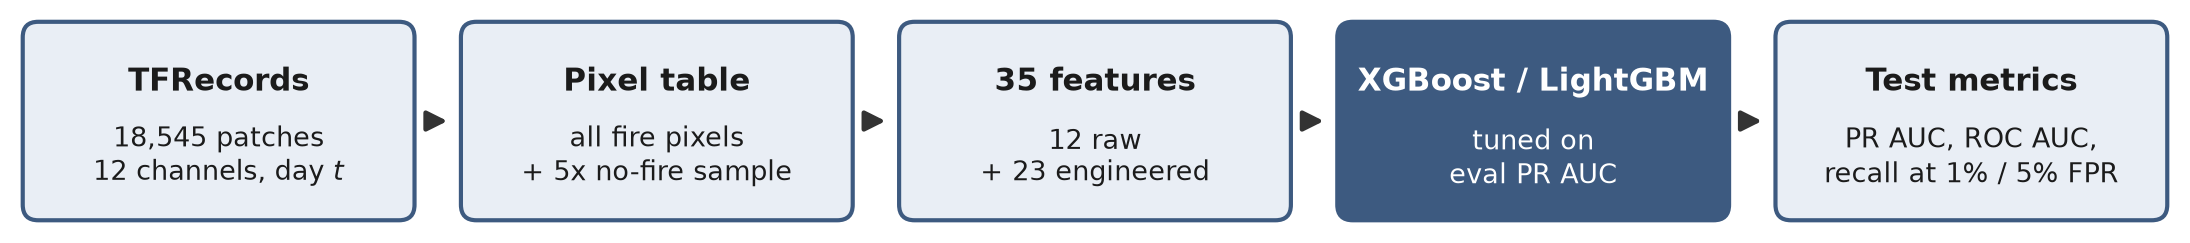
\includegraphics[width=\textwidth]{pipeline.png}
\vspace{0.6em}
\begin{columns}[T]
\column{0.49\textwidth}
\begin{itemize}
\item TFRecords parsed without TensorFlow into $(N,12,64,64)$ arrays
\item Artefacts clipped to fixed physical bounds; wind direction wrapped ($\theta \bmod 360$)
\item Patches are stored south-up; we verified this from slope greenness and downwind spread
\end{itemize}
\column{0.49\textwidth}
\begin{itemize}
\item Training table: every fire pixel + 5:1 no-fire sample = 3.95\,M rows; \texttt{scale\_pos\_weight} = 5
\item 20 random configurations per model, early stopping on eval, best by eval PR AUC
\item Decision threshold: best F1 on eval, applied unchanged to test
\end{itemize}
\end{columns}
\end{frame}

% ---------------------------------------------------------------- Piyush (from paper/sections/methodology.tex)
\begin{frame}{Features: 12 raw + 23 engineered, in five groups}
\begin{columns}[T]
\column{0.56\textwidth}
\footnotesize
\begin{tabular}{@{}l r >{\raggedright\arraybackslash}p{3.7cm}@{}}
\toprule
Group & \# & Engineered examples \\
\midrule
Fire neighbourhood & 10 & fire density (3/5/9\,px), distance, fire upwind \\
Weather & 14 & wind $u$/$v$, VPD, min.\ rel.\ humidity, ERC $\times$ wind \\
Vegetation & 4 & local NDVI mean, std, anomaly \\
Terrain & 5 & slope, aspect, relative elevation \\
Human & 2 & population, $9\times9$ mean \\
\bottomrule
\end{tabular}
\vspace{0.2em}
\footnotesize
\begin{itemize}
\item \texttt{dist\_to\_fire}: univariate AUC 0.866 vs 0.593 for the raw fire mask
\item Most XGBoost gain is in fire features: \texttt{dist\_to\_fire} 32\%, \texttt{prev\_fire\_n9} 23\%, upwind 13.5\%
\end{itemize}
\column{0.42\textwidth}
\centering
\vspace{0.3em}
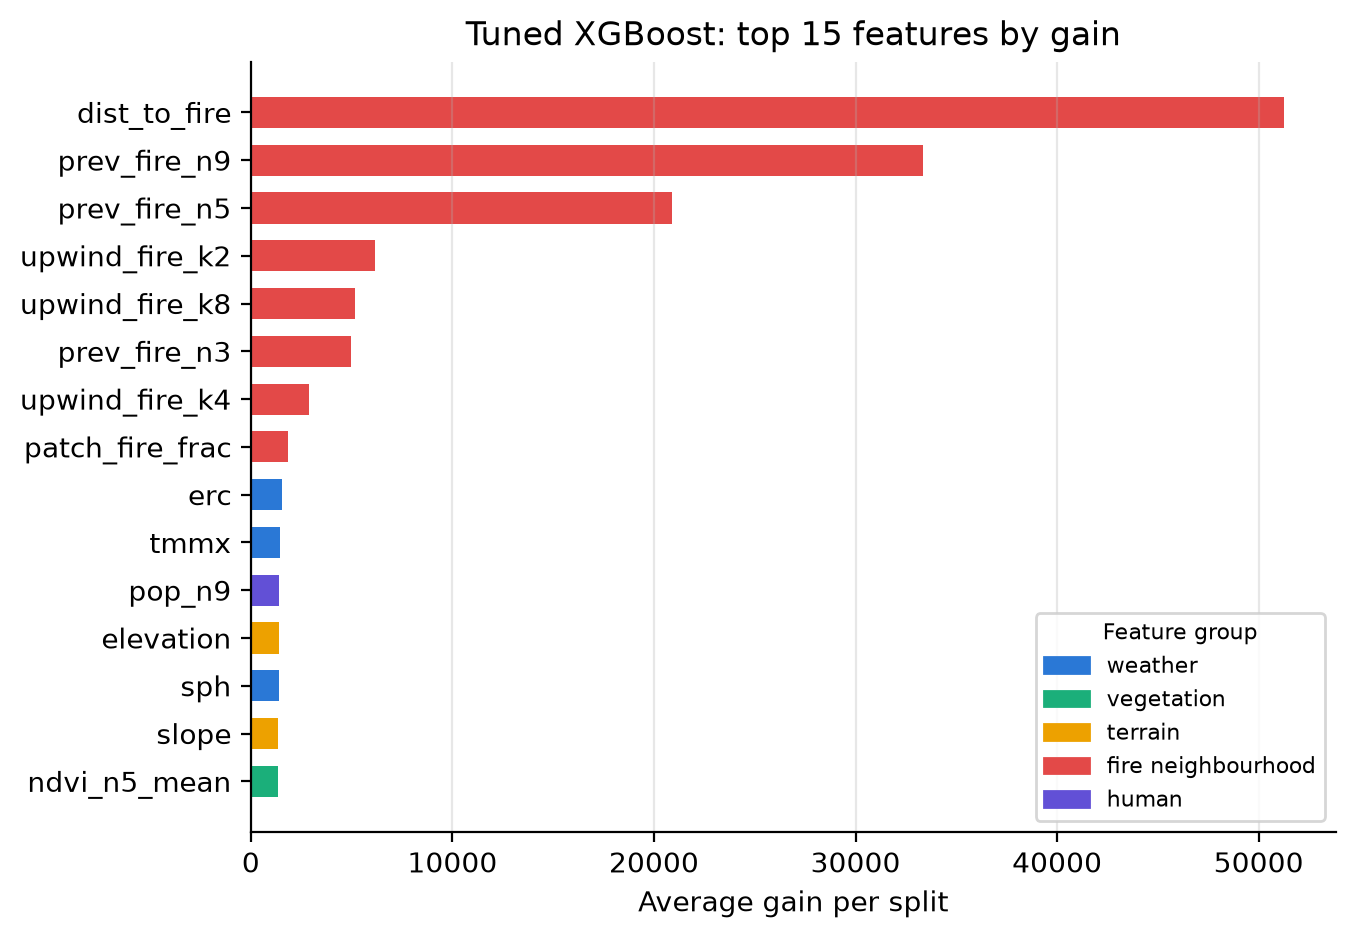
\includegraphics[width=\textwidth]{eval_gain_importance.png}
\end{columns}
\end{frame}

% ---------------------------------------------------------------- Sushant
\begin{frame}{From EDA to features, and what each group is worth}
\begin{columns}[T]
\column{0.44\textwidth}
\begin{itemize}
\item 40\% of new fire is more than 5\,km from day-$t$ fire $\rightarrow$ added \texttt{upwind\_fire\_k8} (ranks 5th of 35 by XGBoost gain)
\item Ablation: dropping fire-neighbourhood features drops PR AUC 0.248 $\rightarrow$ 0.048; vegetation is the most useful environmental group ($-0.009$)
\item Fire features alone: 0.218; environment adds $+0.031$ on top
\end{itemize}
\column{0.54\textwidth}
\centering
\vspace{0.5em}
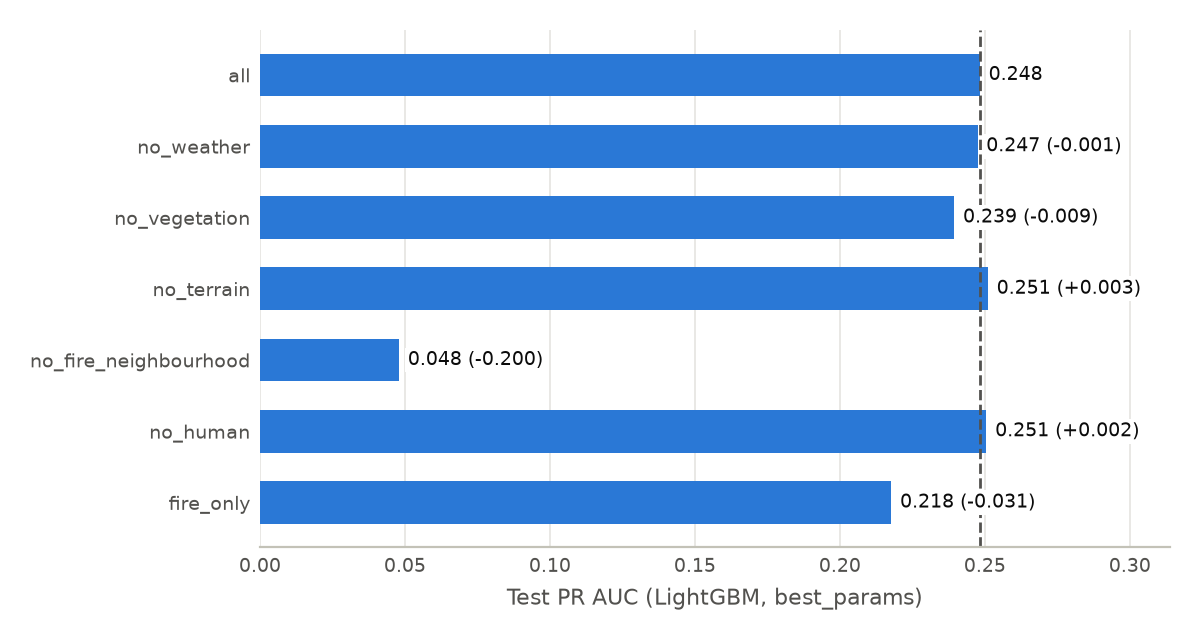
\includegraphics[width=\textwidth]{ablation_pr_auc.png}
\end{columns}
\end{frame}

% ---------------------------------------------------------------- Sachin
\begin{frame}{Engineered features beat every baseline}
\begin{columns}[T]
\column{0.5\textwidth}
\begin{itemize}
\item Tuned XGBoost: \textbf{PR AUC 0.257}, vs 0.145--0.157 for raw-channel models and 0.106 for persistence (LightGBM 0.248)
\item Finds 39\% of next-day fire at 1\% FPR and 68\% at 5\% FPR; highest F1 of all models (0.332)
\item Between Huot et al.'s neighbour RF (0.225) and their CNN (0.284)
\end{itemize}
\column{0.46\textwidth}
\centering
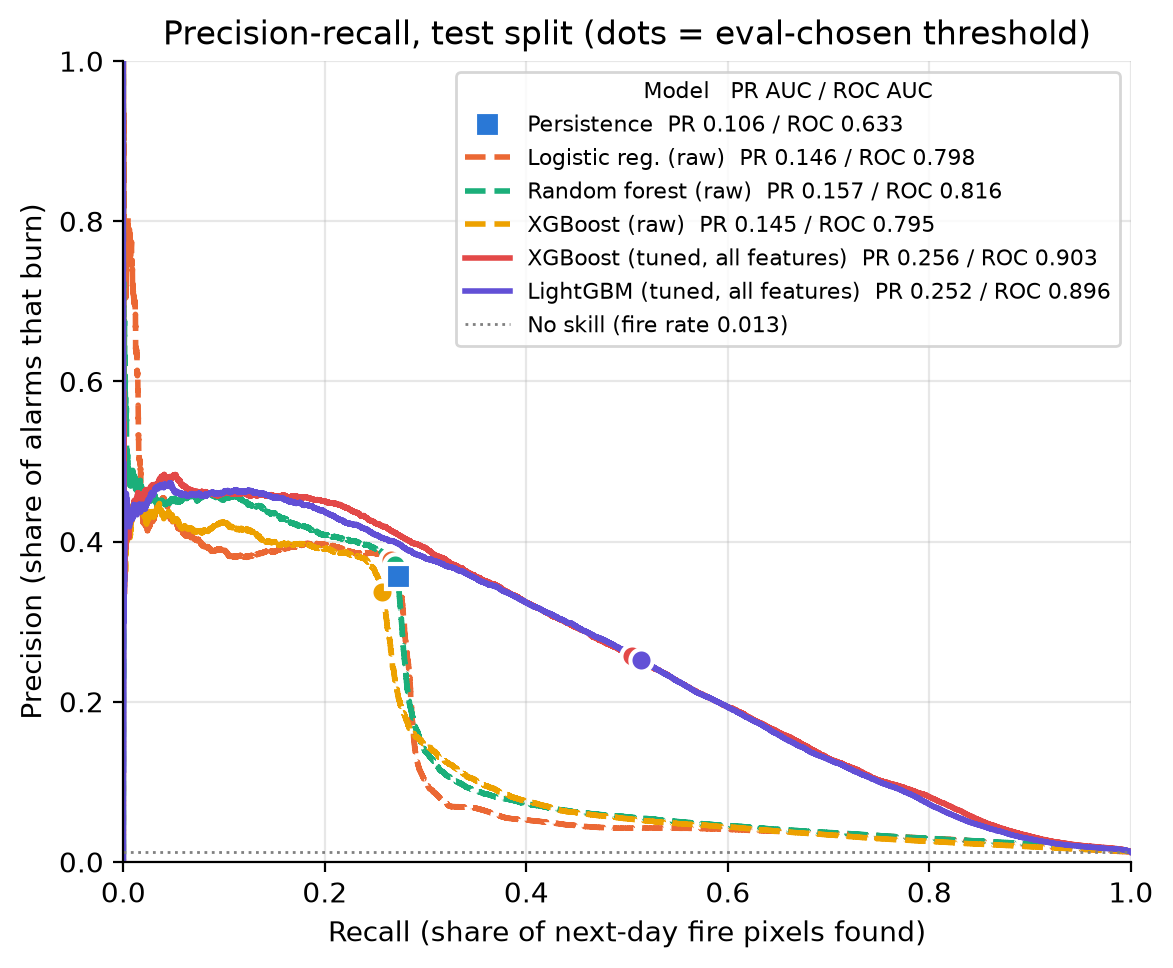
\includegraphics[width=\textwidth]{eval_pr_curves.png}
\end{columns}
\src{All numbers on the test split; F1 at the threshold chosen on eval.}
\end{frame}

% ---------------------------------------------------------------- Priyanshu
\begin{frame}{Where we stand}
\begin{itemize}
\item Our XGBoost on 35 features (12 raw + 23 engineered): 0.257 PR AUC on the same test split (95\% interval over fire events: 0.19--0.33)
\item Between Huot's random forest (0.225) and CNN (0.284), both inside our interval; recent U-Nets reach about 0.35 (Esparza et al.\ 2026 preprint)
\item Tuning moves PR AUC by about 0.01, spatial features by about 0.20. Phase 2: a CNN / U-Net on the whole patch
\end{itemize}
\vspace{0.2em}
\centering
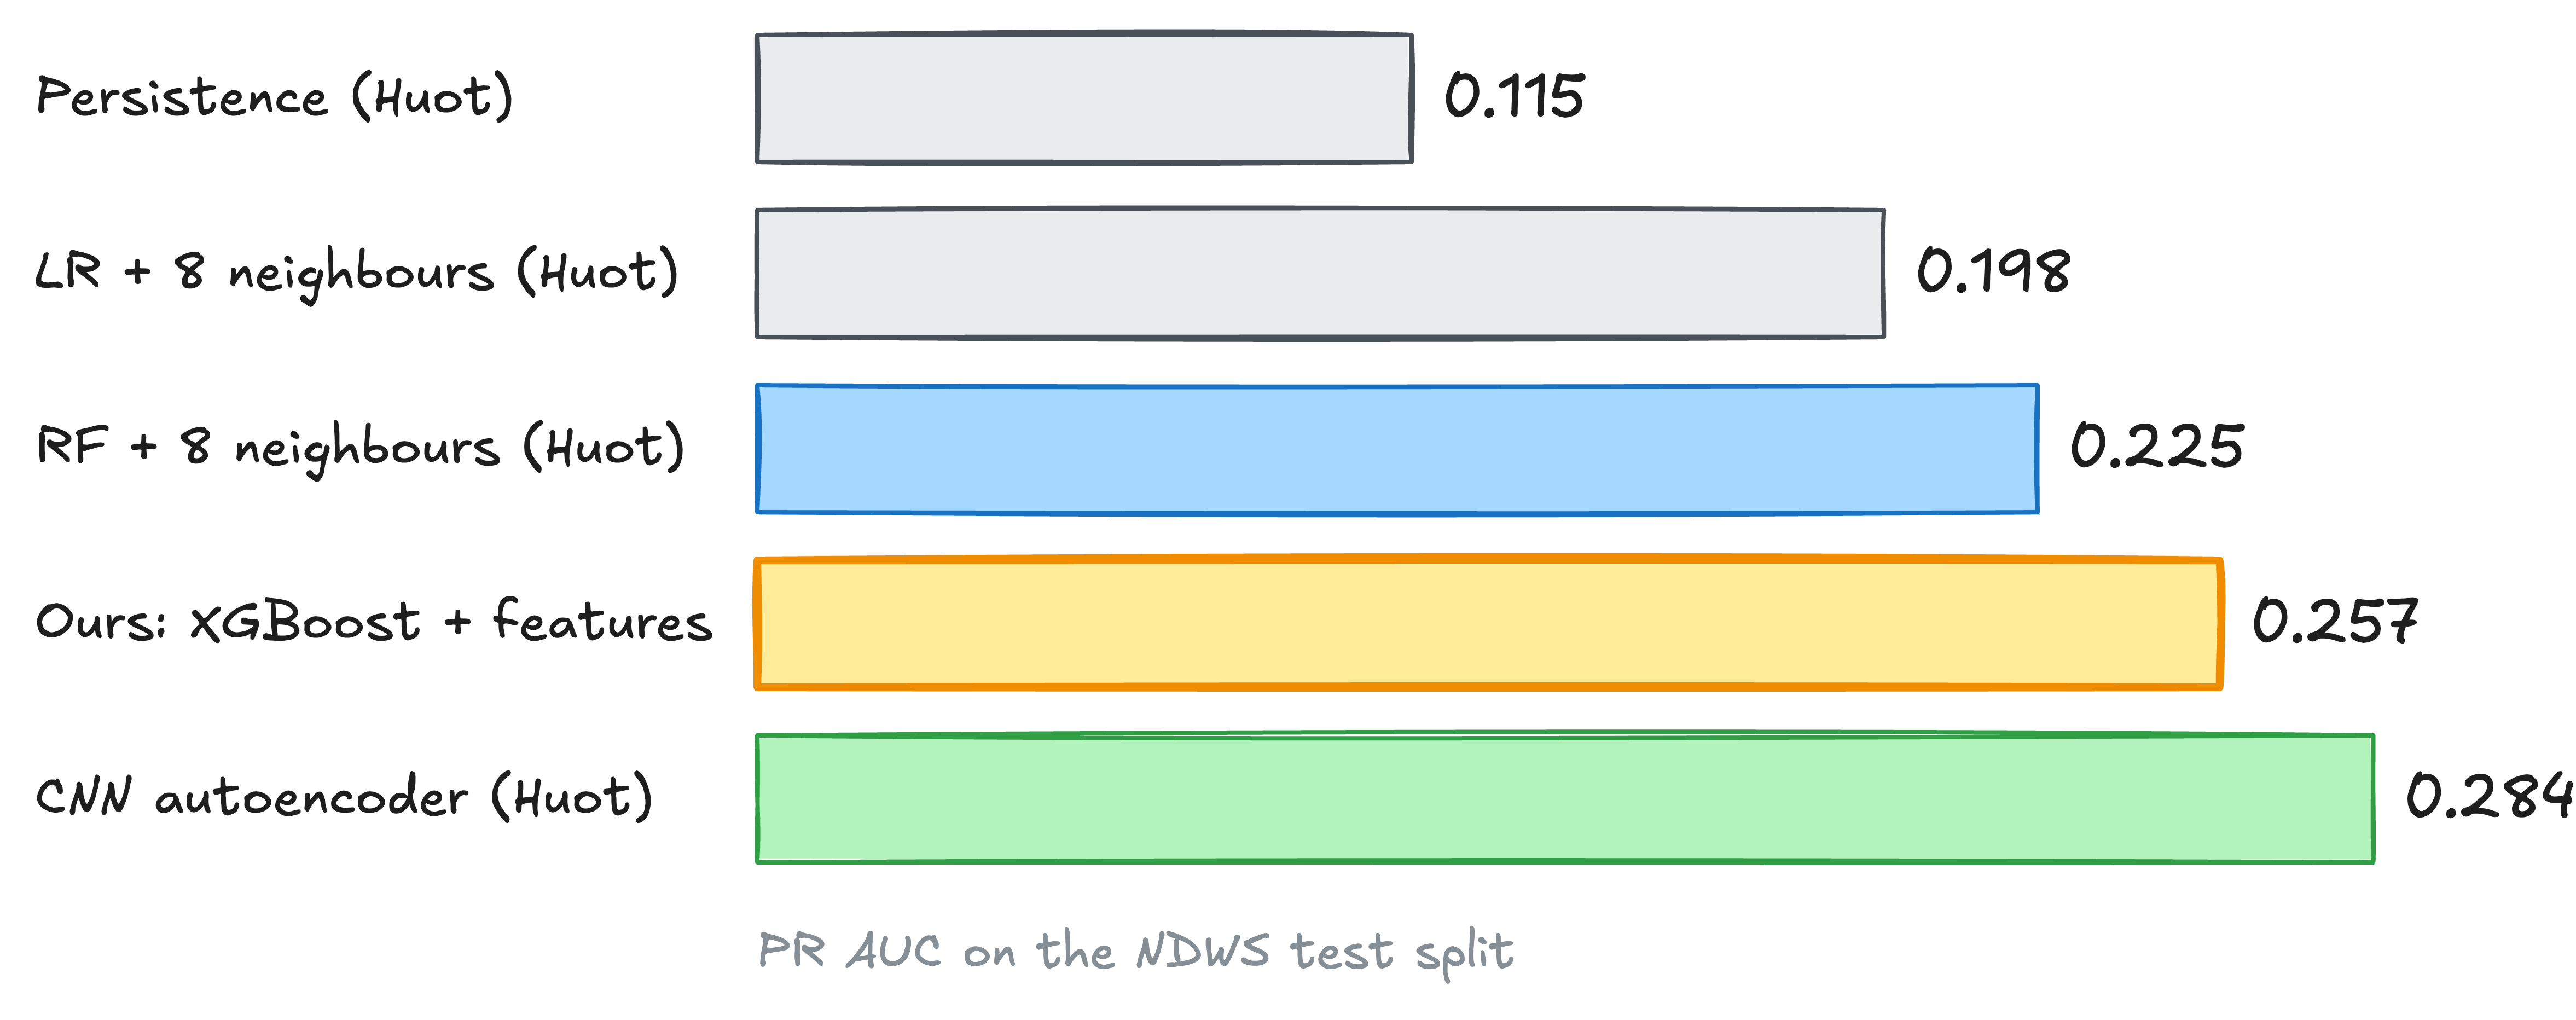
\includegraphics[width=0.68\textwidth]{slide2_where_we_stand.png}
\end{frame}

% ---------------------------------------------------------------- Sachin
\begin{frame}{What the model learned}
\begin{itemize}
\item Predicts a halo around today's fire; fire-neighbourhood features dominate (SHAP 2.29 vs 0.40 for weather)
\item Physically sensible signs: near fire, dry air, strong wind, fire upwind $\rightarrow$ higher risk (ERC is the exception)
\item Pushes risk downwind; train data agrees: downwind/upwind ratio grows from 1.135 (calm) to 3.100 ($\geq$ 8\,m/s)
\end{itemize}
\centering
% top two rows of the 5-row figure
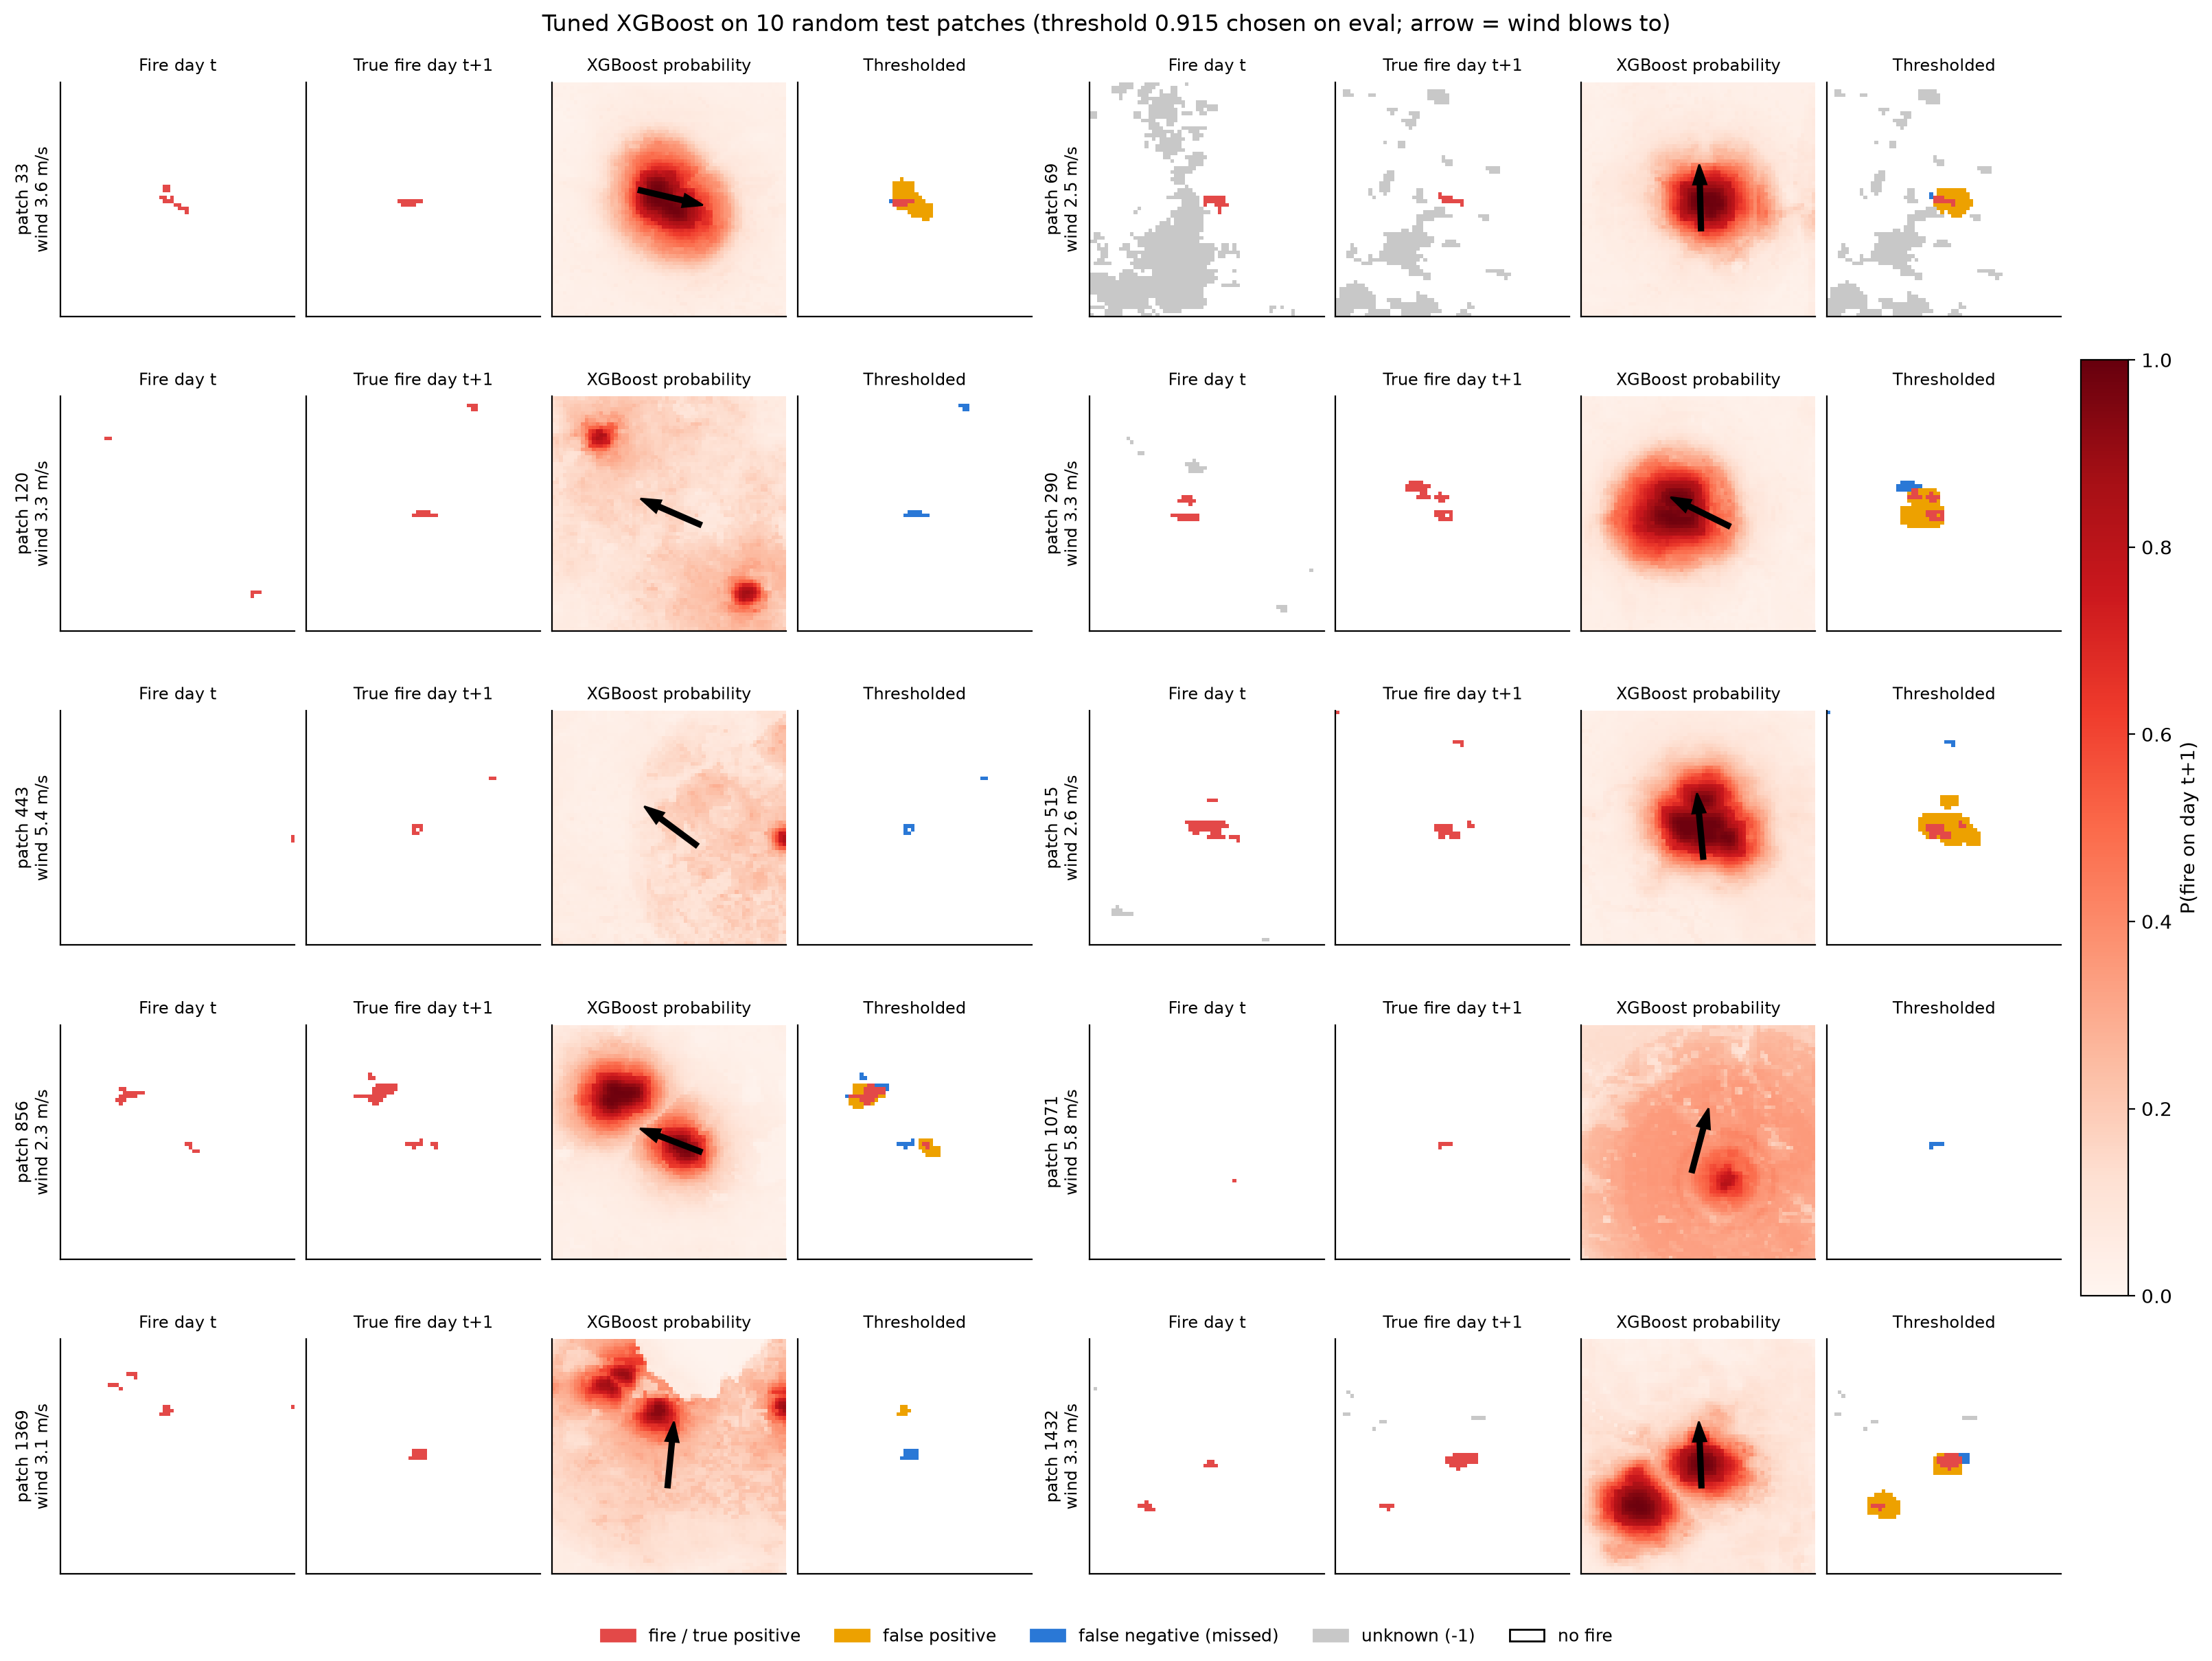
\includegraphics[width=0.8\textwidth, trim=0 535 0 0, clip]{eval_prob_maps.png}
\src{Test patches. Red = fire / true positive, orange = false positive, blue = missed; arrow = wind blows to.}
\end{frame}

% ---------------------------------------------------------------- Sachin
\begin{frame}{Where it fails $\rightarrow$ Phase 2}
\begin{columns}[T]
\column{0.46\textwidth}
\begin{itemize}
\item False alarms around dying fires: 88.8\% within 2\,km of today's fire; only 35.3\% of burning pixels still burn tomorrow
\item Misses long-range spread: recall 0.988 at the fire, 0.648 at 2\,km, 0 beyond 5\,km
\item Fixed-radius halo, no fire-front shape $\rightarrow$ Phase 2: CNN / U-Net that sees the whole patch
\end{itemize}
\column{0.52\textwidth}
\centering
\vspace{0.5em}
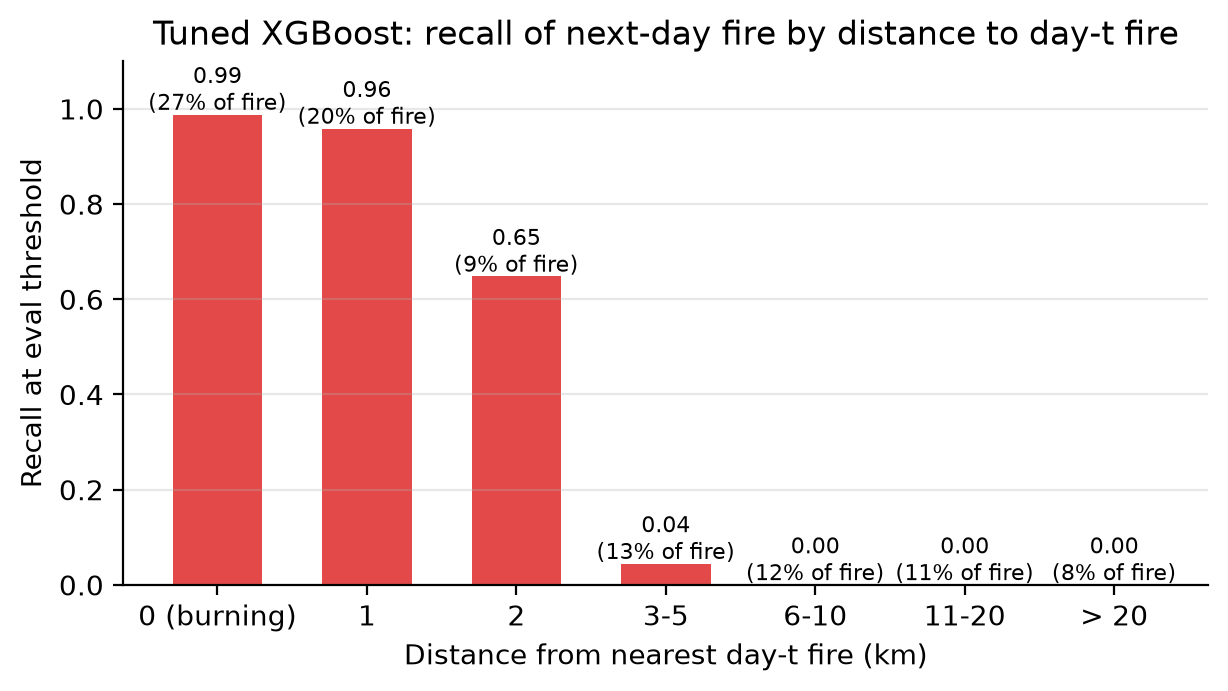
\includegraphics[width=\textwidth]{eval_recall_by_distance.png}
\end{columns}
\end{frame}

% ---------------------------------------------------------------- Piyush
\begin{frame}{Conclusion}
\begin{itemize}
\item A per-pixel model with 23 engineered spatial features reaches test PR AUC \textbf{0.257} (95\% interval over fire events 0.19--0.33), against 0.106 for persistence
\item Huot et al.'s RF (0.225) and CNN (0.284) both lie inside our interval: we land between them, with no claim of a significant difference
\item The signal is spatial: without fire-neighbourhood features PR AUC drops from 0.248 to 0.048; tuning moves it by about 0.01
\item 5\% of the training data gives almost the same eval PR AUC (0.204 vs 0.207): the model is limited by bias, not variance
\item It finds fire at the front (recall 0.96--0.99 within 1\,px) but recall is near 0 beyond 5\,km, where 64\% of missed pixels lie
\item Side finding: the patches are stored south-up, which matters for every wind-based feature
\end{itemize}
\end{frame}

% ---------------------------------------------------------------- Piyush
\begin{frame}{Future work (Phase 2)}
\begin{itemize}
\item \textbf{Whole-patch models:} U-Net / CNN that see the shape of the fire front instead of a fixed-radius halo
\item \textbf{Imbalance-aware losses:} focal loss or class-weighted segmentation loss
\item \textbf{Multi-day inputs:} fire history over several days (WildfireSpreadTS)
\item \textbf{Split leakage check:} whether one fire appears in more than one split (test alone has 40 exact duplicate patches)
\item \textbf{Uncertain labels:} better handling of cloud and smoke ($-1$) pixels than simply ignoring them
\end{itemize}
\end{frame}

% ---------------------------------------------------------------- Piyush
\begin{frame}[plain]
\centering
\vfill
{\color{accent}\Huge\bfseries Thank you\par}
\vspace{0.8em}
{\large Questions?\par}
\vspace{1.5em}
{\small\color{muted}Code, report and figures: \texttt{github.com/harshilv17/next-day-wildfire-spread}\par}
\vfill
\end{frame}

\end{document}
